\documentclass[a4j,10pt,dvipdfmx]{jarticle}
\usepackage{url}
\usepackage[version=3]{mhchem}
\usepackage{siunitx}
\usepackage[dvipdfmx]{graphicx}
\usepackage{pdfpages}
\usepackage{here}
\usepackage{tabularx}
\author{学籍番号2120029, 氏名 政野玄空}
\date{2023年6月4日}
\begin{document}
\section{実験目的}
トランジスタの静特性の測定,バイアス回路の電圧の測定,周波数特性の測定を通してトランジスタ増幅回路の動作を確認し,トランジスタの増幅回路の仕組みを学び理解する.
\section{原理}
\subsection{トランジスタの静特性}
トランジスタはP型半導体とN型半導体と呼ばれる半導体の接触面のPN接合を3層に組み合わせており各層にエミッタ,ベース,コレクタの3つの端子を持つ.Pにはホールと呼ばれるプラス電荷がありNには自由電荷があるため半導体はPからNへの向きへ電流が流れ逆には流れない.
NPN型トランジスタにエミッタ接地方式で電圧をかけたときの図を(\ref{npn})に示す.BE間にはダイオードと同様順方向電圧$V_{BE}$がかけられており,$V_{CE}$がかかっていないとき,E側の自由電子はB端子に流れ込み電流$I_B$となる.
CE間に$V_{CE}$をかけるとE側に存在していた自由電子は中間のP層を越えてC端子に到達する.この電子の流れが電流$I_C$であり,$I_C$の量は$V_CE$が印加されていればその電圧の大小よりも$I_b$によって増減する.
\begin{figure}[H]
  \label{npn}
  \begin{center}
  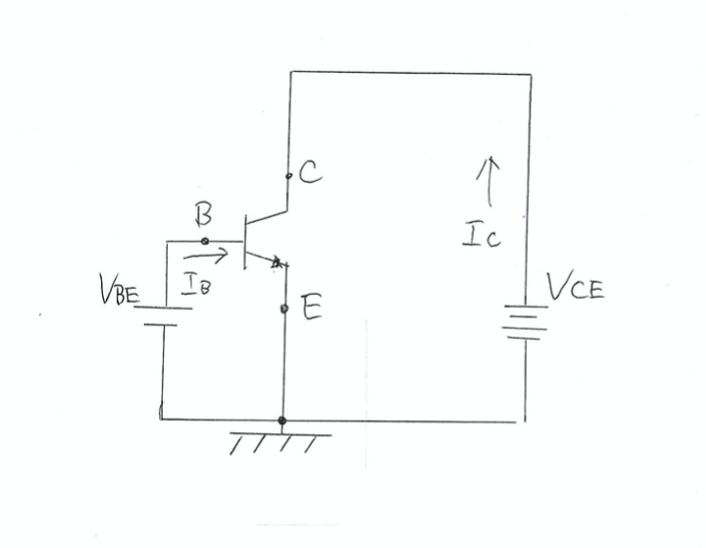
\includegraphics[height=7cm,width=10cm]{NPN.png}
  \caption{NPN型トランジスタにエミッタ接地方式で電圧をかけたときの図}
\end{center}
\end{figure}
$I_C$の電流の最大値は$V_CE$,出力を取り出すための負荷抵抗で決まり,加える$I_B$はわずかになる.よって$I_B$により$I_C$を増幅されることが確認できる.
このときの$I_C$/$I_B$は電流増幅率と呼び$hFE$と表される.
このように各端子にかけられた直流バイアスのいずれかを変化させ測定したものの特性を静特性とよぶ.
\subsection{バイアス回路の確認}
静特性は$I_C$-$V_{CE}$,$I_C$-$I_B$,$I_B$-$V_{BE}$,$V_{BE}$-$V_{CE}$が連動しており,$I_B$,$V_{BE}$が決まれば$I_C$,$V_{CE}$が定まるようになっている.これを利用してバイアス点を定め交流信号を加える.
\begin{figure}[H]
  \label{bias}
  \begin{center}
  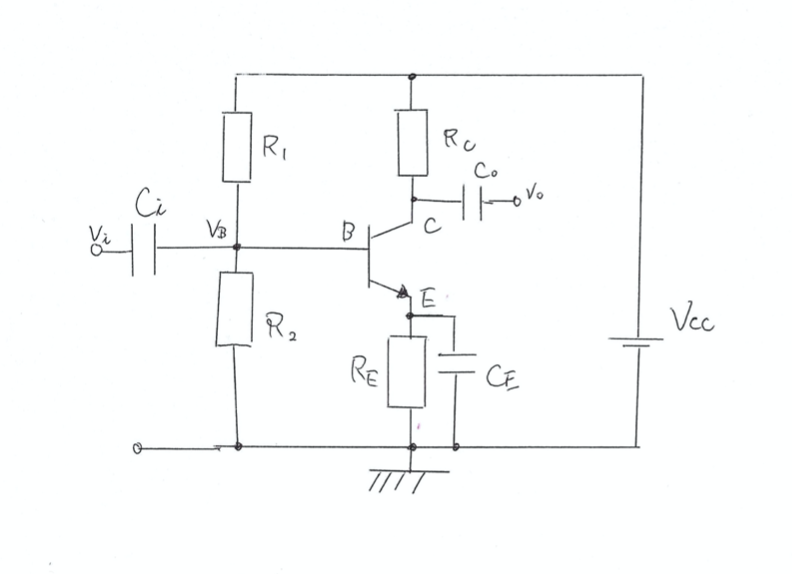
\includegraphics[height=7cm,width=10cm]{bias.png}
  \caption{バイアス増幅回路の図}
\end{center}
\end{figure}
(\ref{bias})のように抵抗によって各所の直流電圧電流比率を一定に保つ構成の回路を電流帰還バイアス回路という.これにはエミッタ抵抗$R_E$が存在することでコレクタ電流の温度による上昇に対し負帰還作用を持ち$R_1$,$R_2$によってベース電位$V_B$が一定に保たれるという特徴がある.
$C_E$は高い増幅率を得るため交流信号に対する負帰還をさける目的で接続されている.
$C_i$,$C_0$はこの増幅回路とは別の前後の回路システムに交流信号のみ伝えるためのバイパスコンデンサである.
増幅度は$C_E$がない場合
\begin{eqnarray}
  \label{z1}
  |A_{V}| = \frac{R_C}{R_E}
\end{eqnarray}
増幅周波数帯での増幅度
\begin{eqnarray}
  \label{z2}
  |A_{V}| = \frac{h_{e}R_{C}}{h_{ie}}
\end{eqnarray}
となる.

\subsection{周波数特性の測定}
アナログ回路では信号の状態を解析するために等価回路モデルが用いられ, 電子回路のような非線形な特性をもつ素子であっても,インピーダンスをもつ素子と理想の電流源を組み合わせ,回路の状態を計算で求めることができるように部品が接続されている.
電流帰還バイアス増幅回路の交流信号に着目した小信号等価回路を解析して,入出力電圧の比から電圧増幅度を求めると
\begin{eqnarray}
  \label{z3}
  |A_{V}| = \frac{v_0}{v_i}= \frac{-(h_{fe}R_C)(1+j\omega{C_E}{R_E})}{h_{ie}+R_E(1+h_{ie})+j\omega{C_E}{R_E}h_{ie}}
\end{eqnarray}
となり,絶対値をとると電圧利得の理論式となり,有利化して実部,虚部の比率をとると位相差の理論値になる.

\section{実験方法}
\subsection{トランジスタの静特性}
NPN型バイポーラトランジスタ2SC1815-Yの静特性を測定する.トランジスタ2SC1815-Y,$R_B$=100kΩ,$C_{po}$=1000pFを回路基板に取り付ける.
直流可変電源とデジタルマルチメーターを(\ref{241})のように回路基板につなぐ.
\begin{figure}[H]
  \label{241}
  \begin{center}
  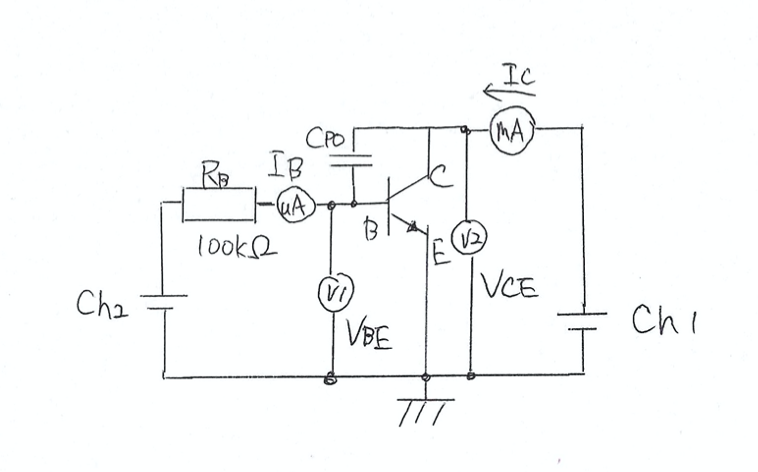
\includegraphics[height=7cm,width=10cm]{241.png}
  \caption{電流帰還バイアス回路の測定点}
\end{center}
\end{figure}
まず$I_B$-$V_{BE}$特性,$I_C$-$I_B$特性について測定する.
Ch1を調整し,$V_CE$が4Vになるように設定する.測定中は常に4Vになるように調整する.
次に$I_C$-$V_{CE}$特性を測定する.$I_B$を10μAになるように2Chを調整する.次にCh1を調整し,$V_CE$=0~12Vの間で変化させ,$I_C$を記録する.その間$I_B$は一定の10μAになるよう調整する.
同様に20,30μAも測定する.

\subsection{バイアス回路の確認}
トランジスタの静特性の実験で測定した結果からバイアス回路を\cite{a}の(3)を参考に設計し実装する.
トランジスタの静特性の結果(\ref{1})より,20μAあたりは$I_C$=3.039,$I_B$=20.059となるので
  
\begin{eqnarray}
  \label{hFE}
  h_{FE}=\frac{3.039}{20.059\times10^{-3}}=151.5[mA]
\end{eqnarray}
同様に(\ref{1})より,$I_{C2}$=4.854,$I_{B2}$=31.932,$I_{C1}$=1.691,$I_{B1}$=11.210となり
\begin{eqnarray}
  \label{hfe}
  h_{fe}=\frac{4.854-1.691}{31.932-11.210\times10^{-3}}=152.6[mA]
\end{eqnarray}
となる.
つづいて$h_{ie}$ を求める.$A_V$は\cite{a}の表2.1より150,$R_C$は\cite{a}の(2.5)と表2.1より2.2kΩ,$h_{fe}$は(\ref{hfe})で求めたので,\cite{a}の(2.6)より

\begin{eqnarray}
  \label{hie}
  h_{ie}=\frac{150\times{2200}}{150}=2238.13[mA]
\end{eqnarray}
\cite{a}の(2.7)より,$I_{B2}$=31.932,$I_{B1}$=11.210,$V_{BE2}$=0.704,$V_{BE1}$=0.678となり
\begin{eqnarray}
  \label{hie2}
  h_{ie}=\frac{0.704-0.678}{31.932-11.210\times10^{-3}}=1254.71[mA]
\end{eqnarray}
$V_{CCE}$ = 7.44 [V]
$I_C$座標軸上のバイアス点$I_{CQ}$を求める.

\begin{eqnarray}
  \label{icq}
  I_{CQ}=\frac{V_1-V_2}{R_C}=1.69[mA]
\end{eqnarray}
$I_B$座標軸上のバイアス点$I_{BQ}$を求める.
\begin{eqnarray}
I_{BQ}=11.08[\mu{A}]
\end{eqnarray}
$V_CC$ = $V_1$ = 12[V]
$V_E$は$V_{CC}$-$V_{CCE}$より4.56[V]
\begin{eqnarray}
R_E = \frac{V_E}{I_{CQ}}=2698.2[Ω]
\end{eqnarray}
\begin{eqnarray}
  \label{r1r2}
  R_1 +R_2= \frac{V_CC}{10/times{I_{BQ}}}=108.3\times10^{3}[Ω]
  \end{eqnarray}
\begin{eqnarray}
  \label{vb}
  V_B = V_E - V_{BEQ} = 4.56+0.678=5.238[V]
\end{eqnarray}

\begin{eqnarray}
  \label{r2}
  R_2 = (R_1+R_2)\frac{V_B}{V_CC}= 47.1\times{10^3} [Ω]
\end{eqnarray}
\begin{eqnarray}
  \label{r1}
  R_1 = 61.2\times{10^{3}}[Ω]
\end{eqnarray}
\begin{eqnarray}
  \label{ce}
  C_E \geq{54.64}[nF]
\end{eqnarray}
\begin{eqnarray}
  \label{ci}
  C_i \geq{0.53}[nF]
\end{eqnarray}
\begin{eqnarray}
  \label{c0}
  C_0 \geq{0.36}[nF]
\end{eqnarray}
がそれぞれ導き出されたので$R_1$に67kΩ,$R_2$に46kΩの抵抗を選んで取り付けた.実測値はそれぞれ67.8352kΩ,46.8978kΩだった.
コンデンサは$C_E$は1mFのものを,$C_i$を100nFのものを直列接続した.実測値はそれぞれ960.6754nF,95.2922μFとなった.
これをもとにバイアス回路を実装し,直流可変電源を12Vになるように流す.
V1~V3とVBを測定し,それぞれの電圧と電流値を算出する.
\subsection{周波数特性の測定}
実装したバイアス回路に直流可変電源を$V_CC$の位置へ接続する.Sig位置に交流電源としてBA信号線,基盤のGND位置に直流可変電源のGNDとBAのGND線をつなぐ.
オシロスコープのCH1を減衰率を1倍にして$v_i$位置に,CH2を減衰率10倍にして$v_o$位置に接続する.オシロスコープは入力結合をACとする.
ファンクションジェネレータの出力の設定をsin波,26mVpp,1kHzにし,バッファアンプの電源を入れる.
直流可変電源を12Vに設定し$V_{CC}$として,直流電圧をかける.
ファンクションジェネレータを出力し,オシロスコープの$v_i$,$v_0$を記録し,利得を求めグラフを作成する.
同様に周波数を100kHzから100Hzまで測定する.
各周波数においてオシロスコープで$\delta{t}$を記録する.
位相差を求めグラフにする.
\section{結果}
\subsection{トランジスタの静特性}
$I_C$ - $V_{CE}$ 特性,$I_C$ - $I_B$ 特性,$I_B$ - $V_{BE}$ 特性の測定データをそれぞれ表とグラフで示す.
\begin{table}[H]
  \label{1}
  \begin{center}
  \caption{$V_{CE}$が4Vのときの$I_C$ - $I_B$,$I_B$ - $V_{BE}$特性}
  \begin{tabular}{cccc} \\
  \hline
  $I_B$[µA] & $I_C$[mA] & $V_{BE}$[V] & $V_{CE}$[V] \\
  17 & 0 & 0 & 0 \\
  0.000  & 0.000  & 0.001  & 4.001  \\
  0.020  & 0.000  & 0.298  & 4.001  \\
  0.250  & 0.030  & 0.570  & 3.998  \\
  2.603  & 0.382  & 0.640  & 3.962  \\
  5.405  & 0.806  & 0.660  & 3.918  \\
  8.293  & 1.245  & 0.670  & 3.873  \\
  11.210  & 1.691  & 0.678  & 4.020  \\
  14.157  & 2.139  & 0.683  & 3.981  \\
  17.106  & 2.589  & 0.688  & 3.935  \\
  20.059  & 3.039  & 0.692  & 3.889  \\
  23.020  & 3.490  & 0.696  & 3.943  \\
  25.988  & 3.944  & 0.699  & 3.896  \\
  28.959  & 4.398  & 0.701  & 3.850  \\
  31.932  & 4.854  & 0.704  & 4.003  \\
  34.909  & 5.328  & 0.706  & 4.486  \\
  37.887  & 5.774  & 0.708  & 3.986  \\
  40.869 & 6.231 & 0.709 & 3.984 \\
   \hline
  \end{tabular}
  \end{center}
  \end{table}
  \begin{table}[H]
  \label{2}
  \begin{center}
  \caption{$I_B$が30[µA]のときの$I_C$ - $V_{CE}$特性}
  \begin{tabular}{ccc} \\
  \hline
  IB[µA] & IC[mA] & VCE[V] \\ \hline
  30.020  & 0.018  & 0.005  \\
  30.059  & 1.088  & 0.089  \\
  29.834  & 2.616  & 0.133  \\
  29.726  & 3.970  & 0.194  \\
  29.714  & 4.390  & 0.351  \\
  29.708  & 4.410  & 0.549  \\
  29.712  & 4.433  & 1.147  \\
  29.714  & 4.446  & 1.545  \\
  29.722  & 4.474  & 2.542  \\
  29.727  & 4.503  & 3.539  \\
  29.740  & 4.547  & 5.534  \\
  29.755  & 4.604  & 7.528  \\
  29.780  & 4.653  & 9.522  \\
  29.808  & 4.704  & 11.518  \\
  29.822  & 4.732  & 12.015  \\ \hline
  \end{tabular}
  \end{center}
  \end{table}
  \begin{table}[H]
  \label{3}
  \begin{center}
  \caption{$I_B$が20[µA]のときの$I_C$ - $V_{CE}$特性}
  \begin{tabular}{ccc} \\
  \hline
  IB[µA] & IC[mA] & VCE[V] \\ \hline
  20.094  & 0.0015 & 0.003 \\
  19.242  & 0.962  & 0.102  \\
  20.000  & 2.351  & 0.160  \\
  19.956  & 2.951  & 0.299  \\
  19.952  & 2.964  & 0.497  \\
  19.953  & 2.971  & 0.696  \\
  19.956  & 2.975  & 0.896  \\
  19.956  & 2.983  & 1.295  \\
  19.958  & 2.988  & 1.494  \\
  19.960  & 2.992  & 1.694  \\
  19.962  & 3.006  & 2.693  \\
  19.970  & 3.034  & 4.689  \\
  19.991  & 3.068  & 6.686  \\
  20.006  & 3.105  & 9.681  \\
  20.029  & 3.137  & 11.678  \\
  20.034  & 3.145  & 12.070  \\ \hline
  \end{tabular}
  \end{center}
  \end{table}
  \begin{table}[H]
  \label{4}
  \begin{center}
  \caption{$I_B$が10[µA]のときの$I_C$ - $V_{CE}$特性}
  \begin{tabular}{ccc} \\
  \hline
  IB[µA] & IC[mA] & VCE[V] \\ \hline
  10.387 & 0.0085 & 0.002 \\
  10.361 & 0.2338 & 0.077 \\
  10.0725 & 0.767 & 0.122 \\
  9.944 & 1.274 & 0.171 \\
  9.912 & 1.456 & 0.252 \\
  9.912 & 1.468 & 0.351 \\
  9.912 & 1.47 & 0.45 \\
  9.912 & 1.471 & 0.55 \\
  9.913 & 1.472 & 0.65 \\
  9.912 & 1.474 & 0.75 \\
  10.234 & 1.522 & 0.845 \\
  10.235 & 1.529 & 1.844 \\
  10.236 & 1.535 & 2.843 \\
  10.239 & 1.541 & 3.843 \\
  10.242 & 1.547 & 4.842 \\
  10.245 & 1.552 & 5.841 \\
  10.25 & 1.559 & 6.84 \\
  10.255 & 1.564 & 7.84 \\
  10.26 & 1.57 & 8.83 \\
  10.262 & 1.574 & 9.838 \\
  10.264 & 1.579 & 10.838 \\
  10.267 & 1.584 & 11.838 \\
  10.252 & 1.584 & 12.056 \\ \hline
  \end{tabular}
  \end{center}
  \end{table}
  \begin{figure}[H]
    \begin{center}
      \label{b-vbe}
    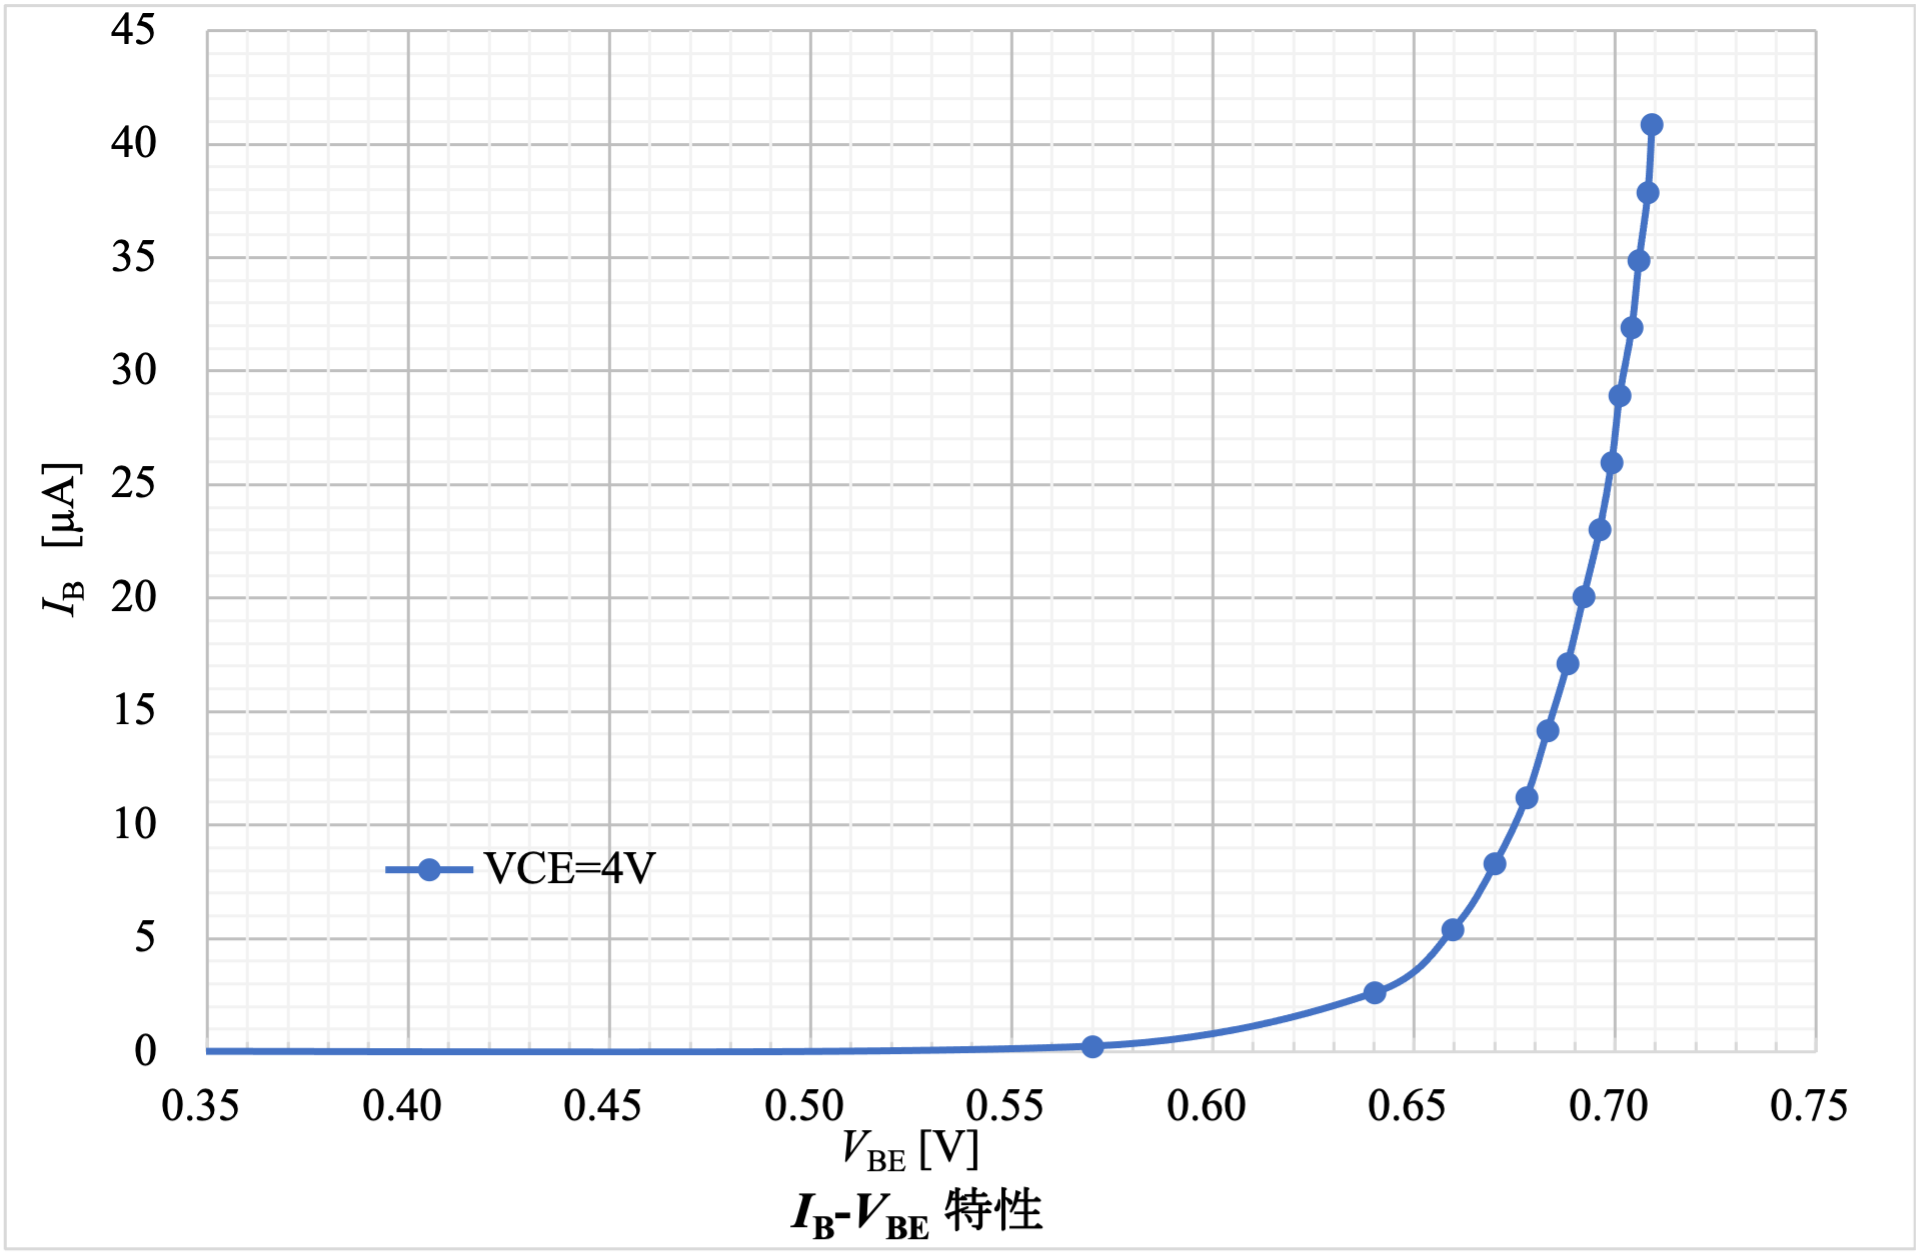
\includegraphics[height=7cm,width=10cm]{4vibvbe.png}
    \caption{$V_{CE}$が4Vのときの$I_B$ - $V_{BE}$特性}
  \end{center}
  \end{figure}
  \begin{figure}[H]
    \begin{center}
      \label{ic-ib}
    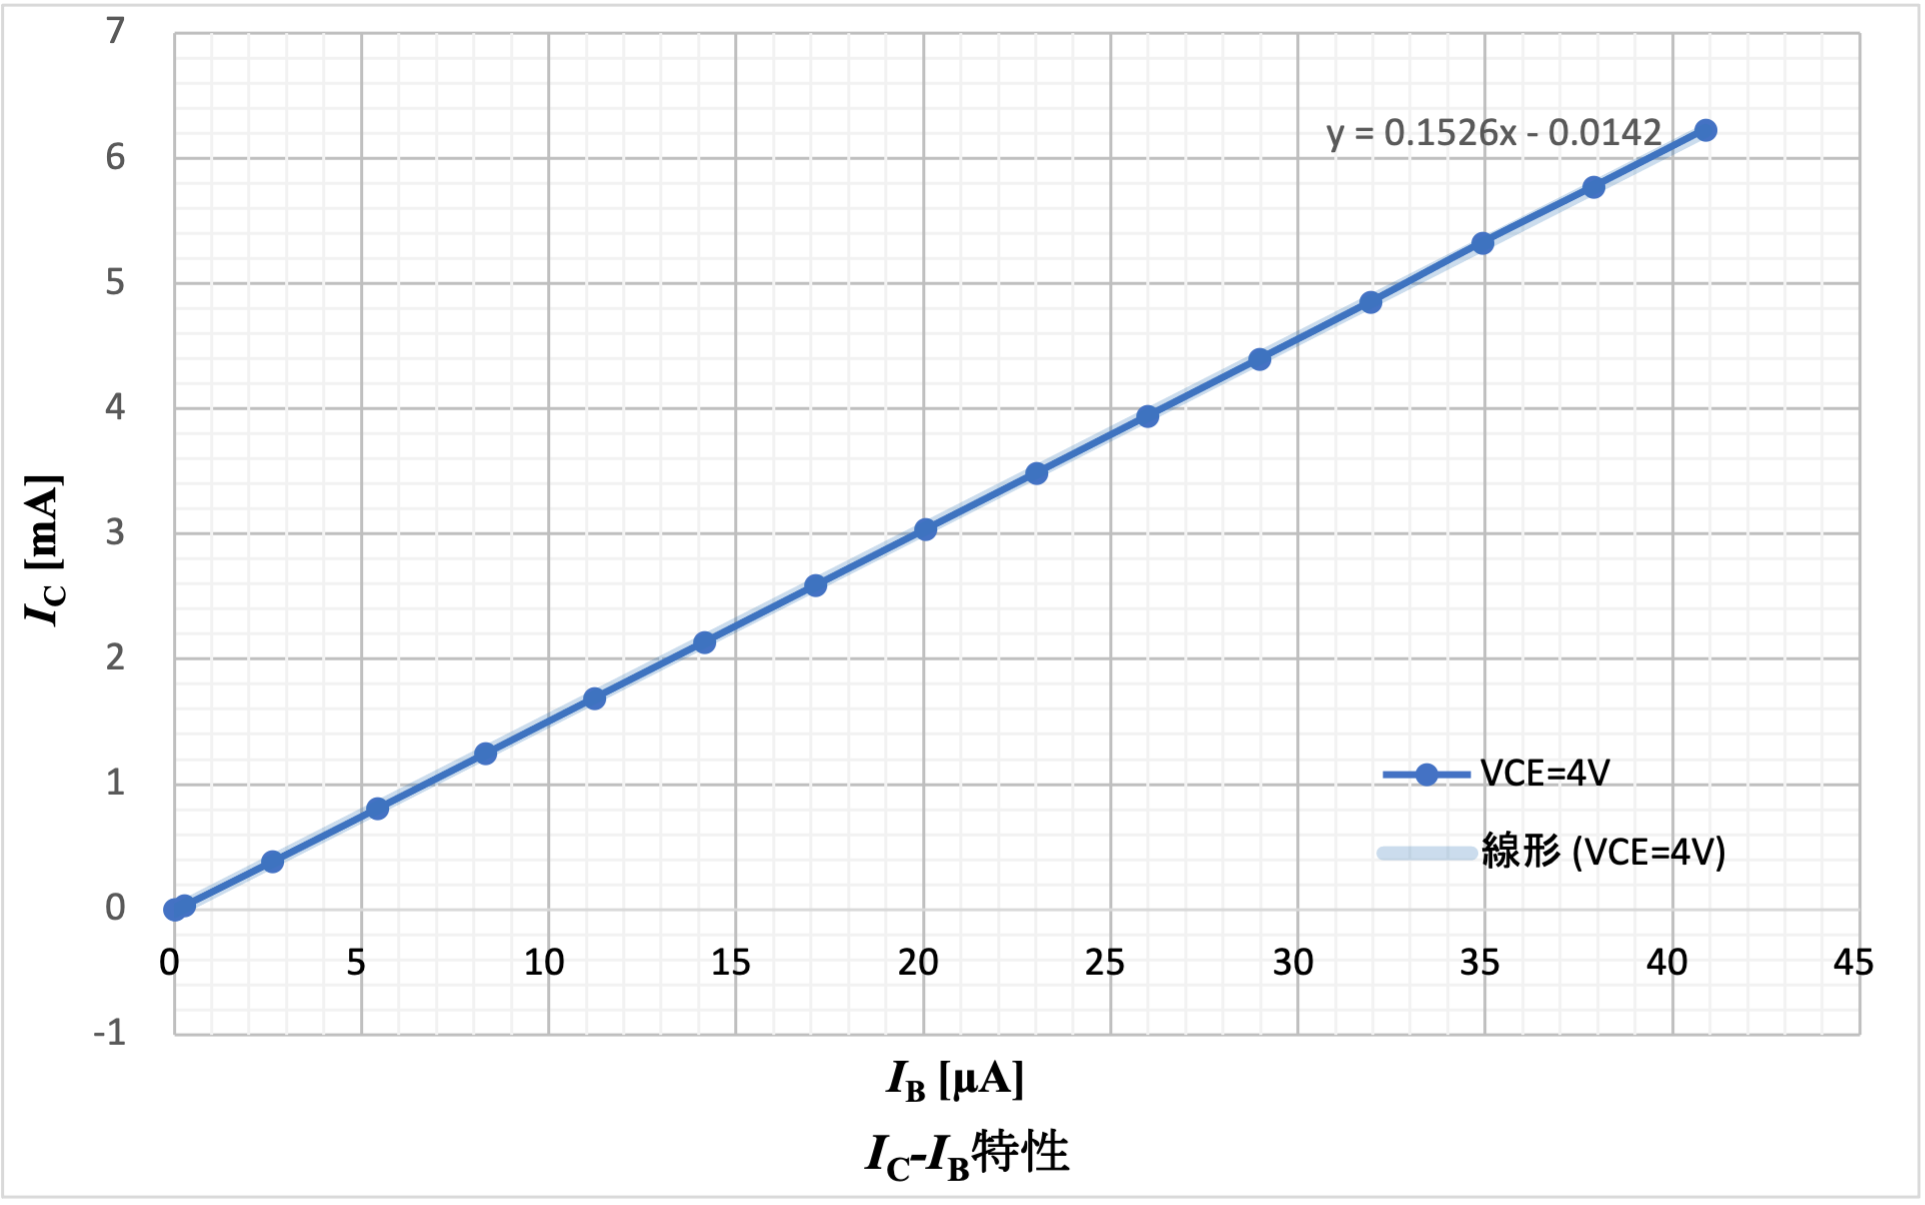
\includegraphics[height=7cm,width=10cm]{v4icib.png}
    \caption{$V_{CE}$が4Vのときの$I_C$ - $I_B$特性}
  \end{center}
  \end{figure}
  \begin{figure}[H]
    \begin{center}
    \label{1030}
    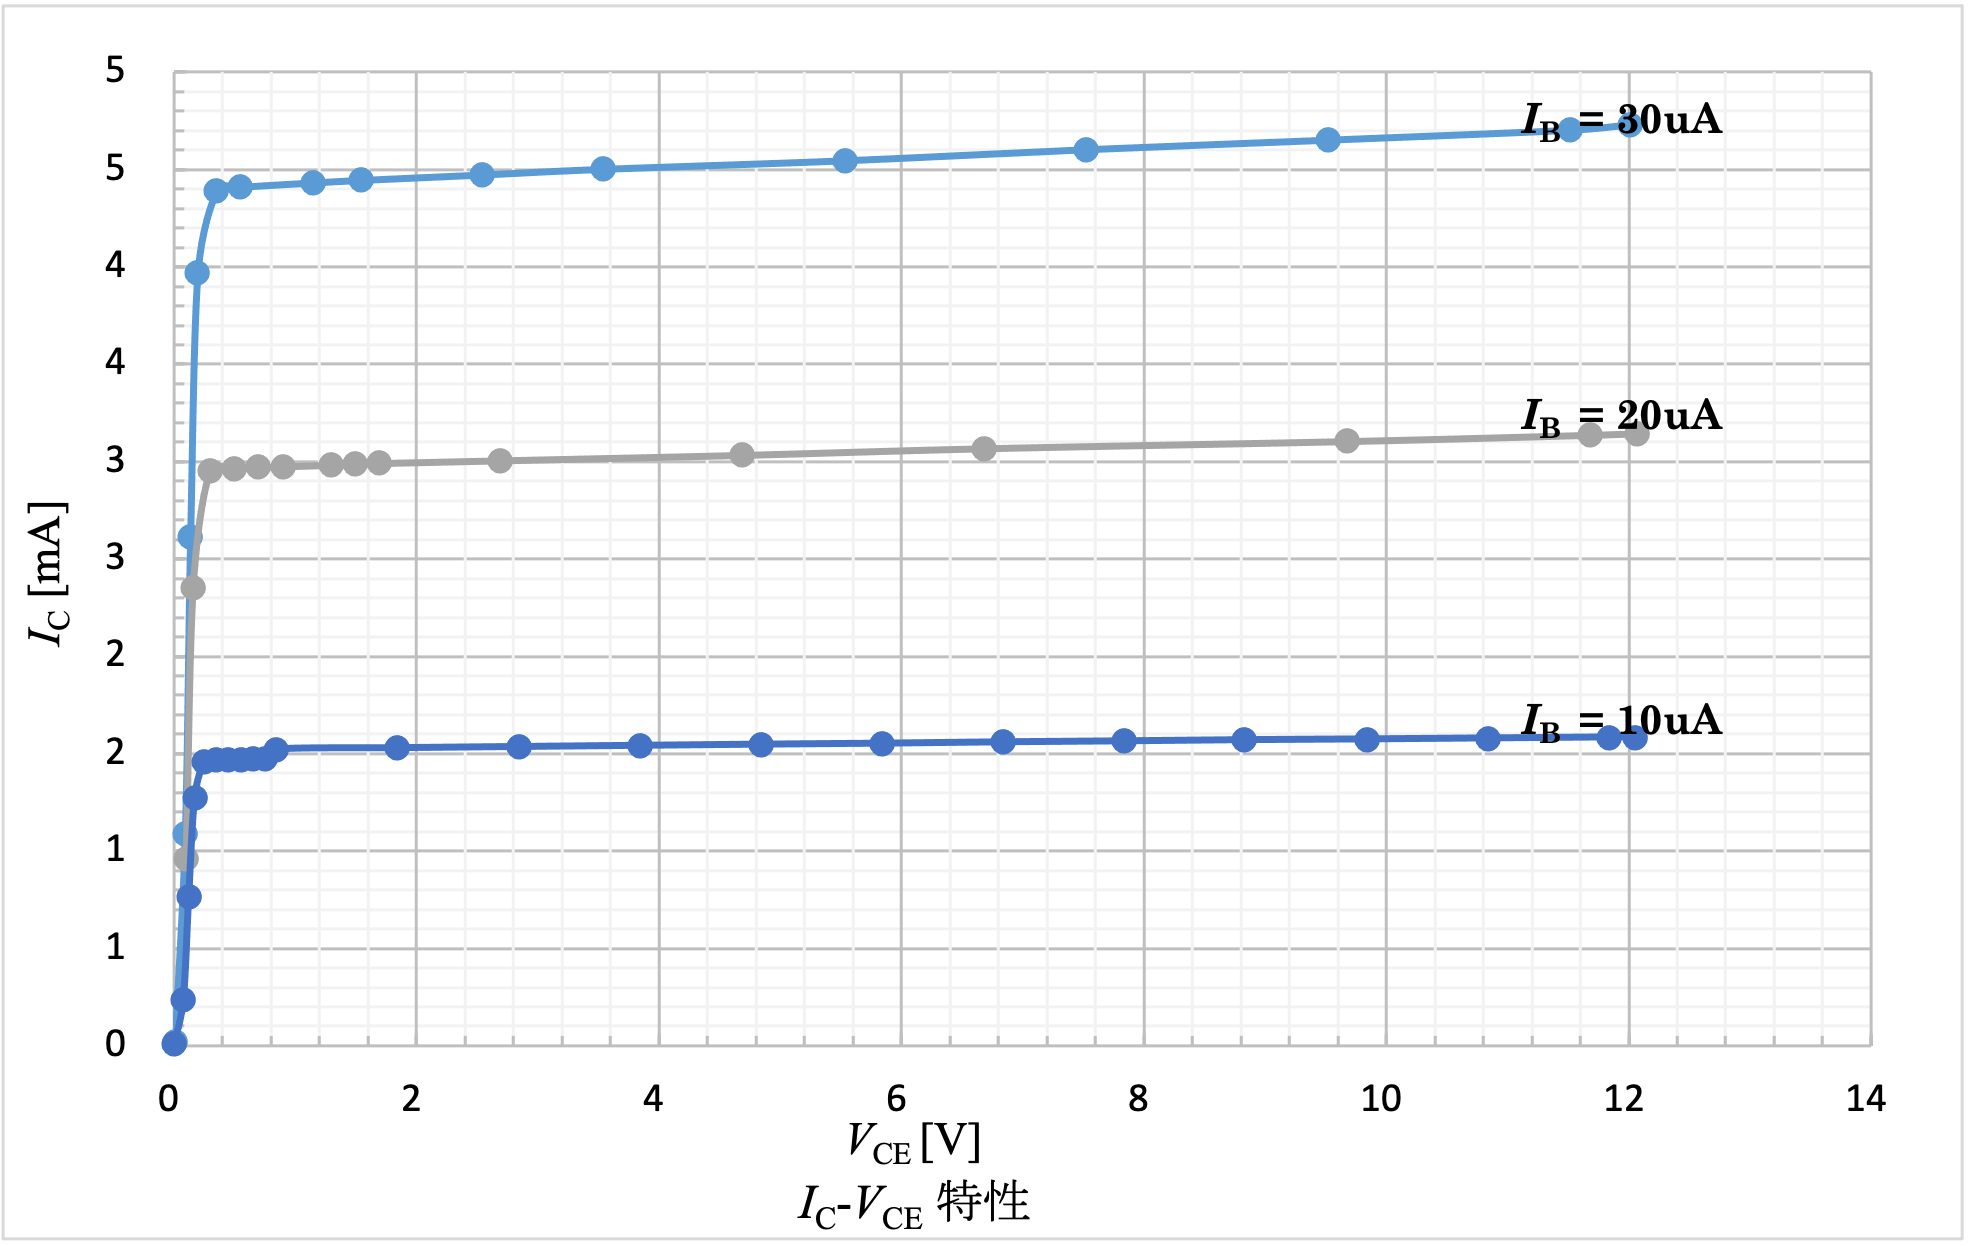
\includegraphics[height=7cm,width=10cm]{icvce1030.png}
    \caption{$I_B$が10[µA],20[µA],30[µA]のときの$I_C$ - $V_{CE}$特性}
  \end{center}
  \end{figure}
\subsection{バイアス回路の確認}
実装したバイアス回路の実測値を測定し,設計時の値と比較する.
\begin{table}[H]
  \label{5}
  \begin{center}
  \caption{バイアス回路の設計時の値と実測値}
  \begin{tabular}{cccc} \\
  \hline
   & 設計時の値 & 実測値 & 差分\\\hline
  V1 & 12V & 12V & 0V \\
  V2 & 8.23V & 8.775V & 0.495V\\
  V3 & 4.56V & 3.98V & -0.58V\\
  VCEQ & 3.72V & 4.795V & 1.075V\\ 
  VB & 5.238& 4.633 & -0.605 \\
  ICQ & 1.69mA & 1.46mA&-0.23mA \\
  IBQ & 11.08µA& 9.548µA & -1.532µA\\
  IEQ & 1.69mA& 1.49mA& -0.22mA \\
  \hline
  \end{tabular}
  \end{center}
  \end{table}
\subsection{周波数特性の測定}
周波数特性の測定結果を表に示す.
\begin{table}[H]
  \label{6}
  \begin{center}
  \caption{周波数特性の測定}
  \begin{tabular}{|l|l|l|l|l|l|l|}
  \hline
      &vi=15mVppと & \multicolumn{2}{|c|}{}& & vi基準の & \\
      &するための & \multicolumn{2}{|c|}{実効値(RMS)} & 実測利得 & voとの & 実測位相差\\
      &FG出力値 &\multicolumn{2}{|c|}{} &&時間差& \\ \hline
      f [Hz] & Fgout [mVpp] & vi[mV] & vo[V] & |Av| [dB] & Δt [us] & φ[deg.]\\ \hline
      100 & 17.7 & 5.3  & 0.448 & 38.62 & -3840 & -138.24 \\ \hline
      200 & 16.3 & 5.3  & 0.54 & 40.29 & -2110 & -151.92\\ \hline
      500 & 15.0 & 5.2  & 0.577 & 40.95 & -906.0 & -163.08\\ \hline
      1000 & 14.7 & 5.1  & 0.59 & 41.12 & -463.0 & -166.68\\ \hline
      2000 & 14.6 & 5.2  & 0.588 & 41.13 & -235.0 & -169.2\\ \hline
      5000 & 14.4 & 5.1  & 0.583 & 41.16 & -95.00 & -171\\ \hline
      10000 & 14.4 & 5.1  & 0.583 & 41.16 & -48.15 & -173.34 \\ \hline
      20000 & 14.5 & 5.1  & 0.587 & 41.15 & -24.00 & -172.8\\ \hline
      50000 & 14.4 & 5.1  & 0.585 & 41.19 & -9.50 & -171\\ \hline
      100000 & 14.4 & 5.1  & 0.59 & 41.22 & -4.800 & -172.8\\ \hline
      200000 & 14.4 & 5.1  & 0.59 & 41.27 & -2.400 & -172.8\\ \hline
  \end{tabular}
\end{center}
\end{table}
次に理論利得を示す.
\begin{table}[H]
  \label{7}
  \begin{center}
  \caption{理論利得と理論位相差}
  \begin{tabular}{|l|l|l|}
  \hline
  FG出力値&理論利得 & 理論位相差 \\ \hline
  f [Hz]&|Av| [dB] & φ[deg.] \\ \hline
  100&39.85197898 & -131.487869 \\ \hline
  200&42.27675197 & -150.3866871 \\ \hline
  500&43.29704887 & -167.1728582 \\ \hline
  1000&43.46454058 & -173.503682 \\ \hline
  2000&43.5074427 & -176.7411955 \\ \hline
  5000&43.51953164 & -178.6952769 \\ \hline
  10000&43.52126138 & -179.3475525 \\ \hline
  20000&43.52169393 & -179.6737655 \\ \hline
  50000&43.52181505 & -179.869505 \\ \hline
  100000&43.52183235 & -179.9347524 \\ \hline
  200000&43.52183668 & -179.9673762 \\ \hline
\end{tabular}
\end{center}
\end{table}
それぞれの利得と位相差を周波数を横軸にグラフ化すると以下のようになった.
\begin{figure}[H]
  \label{rito}
  \begin{center}
  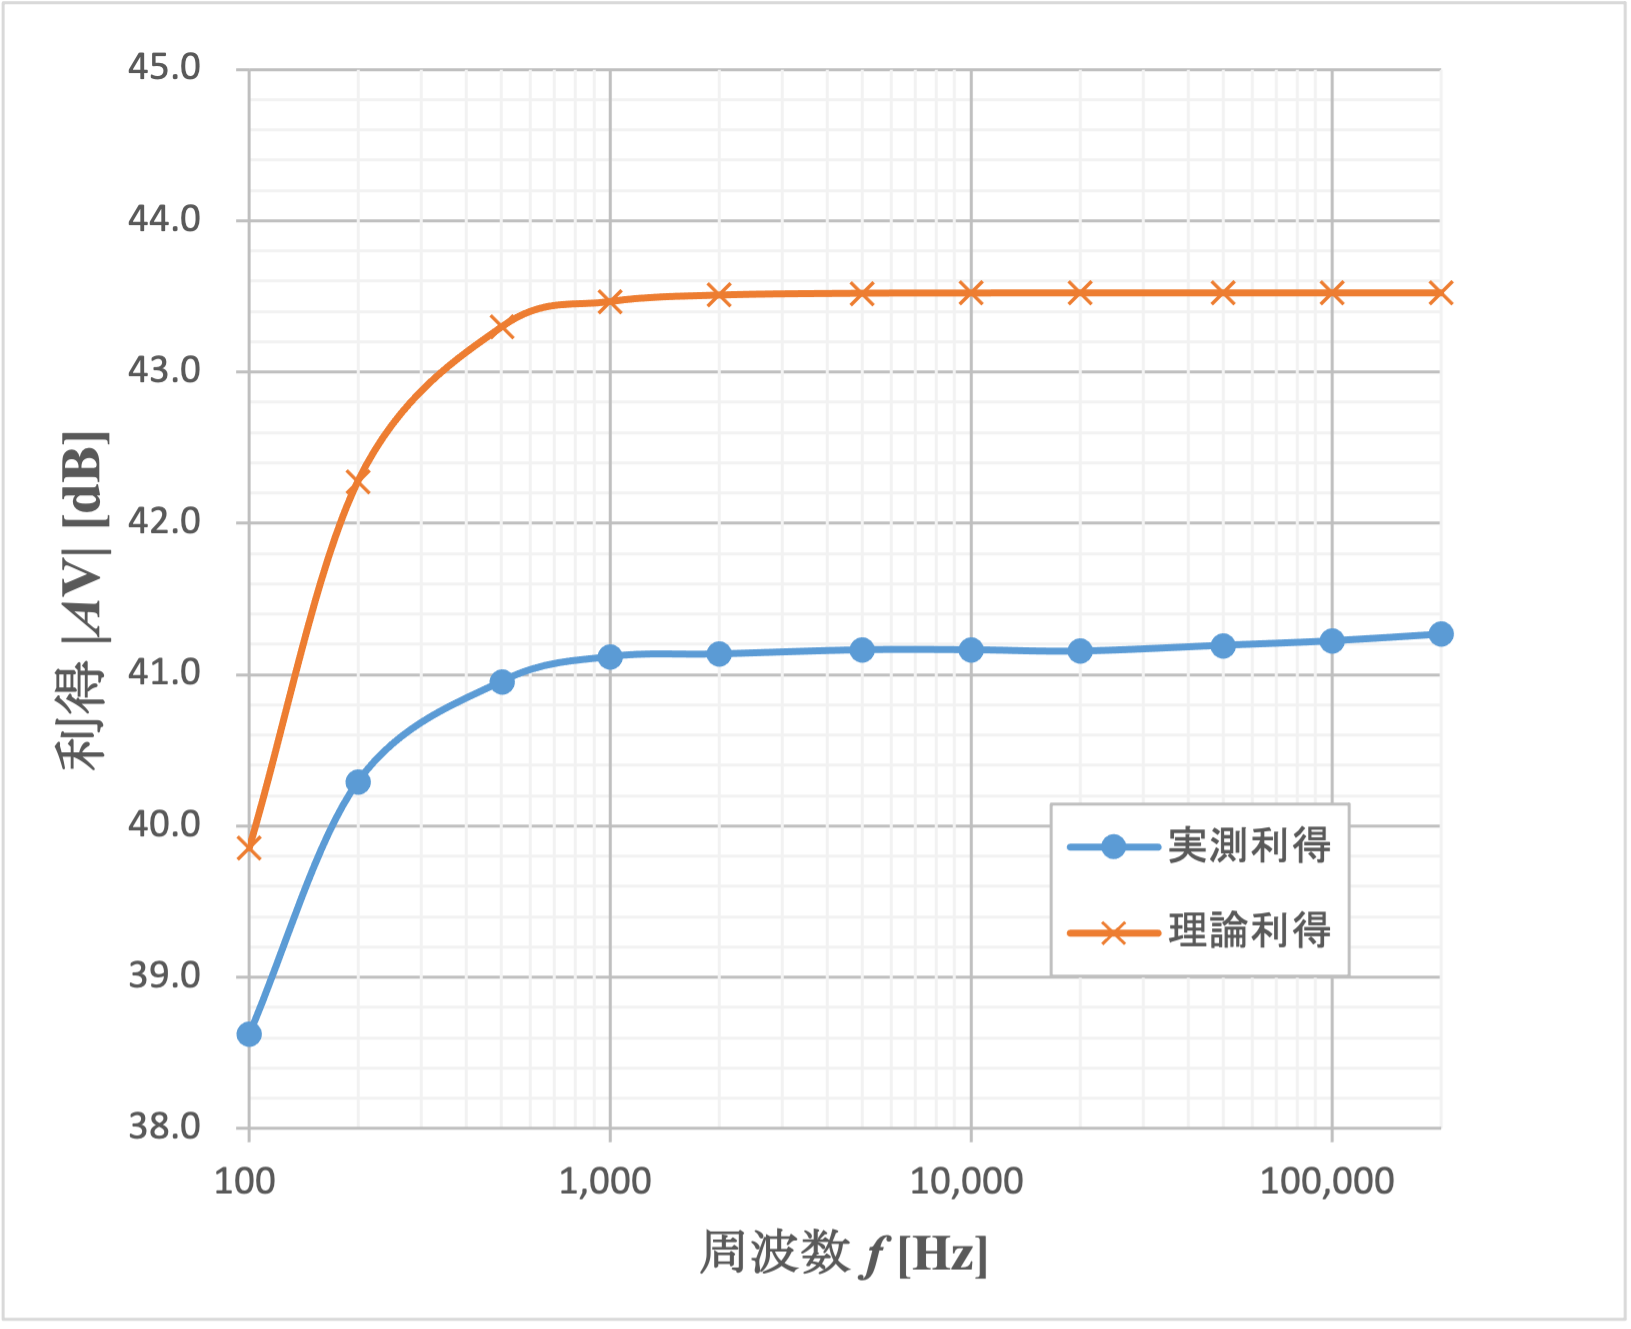
\includegraphics[height=7cm,width=10cm]{ritoku.png}
  \caption{利得の理想値と実測値のグラフ}
\end{center}
\end{figure}
\begin{figure}[H]
  \label{syuha}
  \begin{center}
  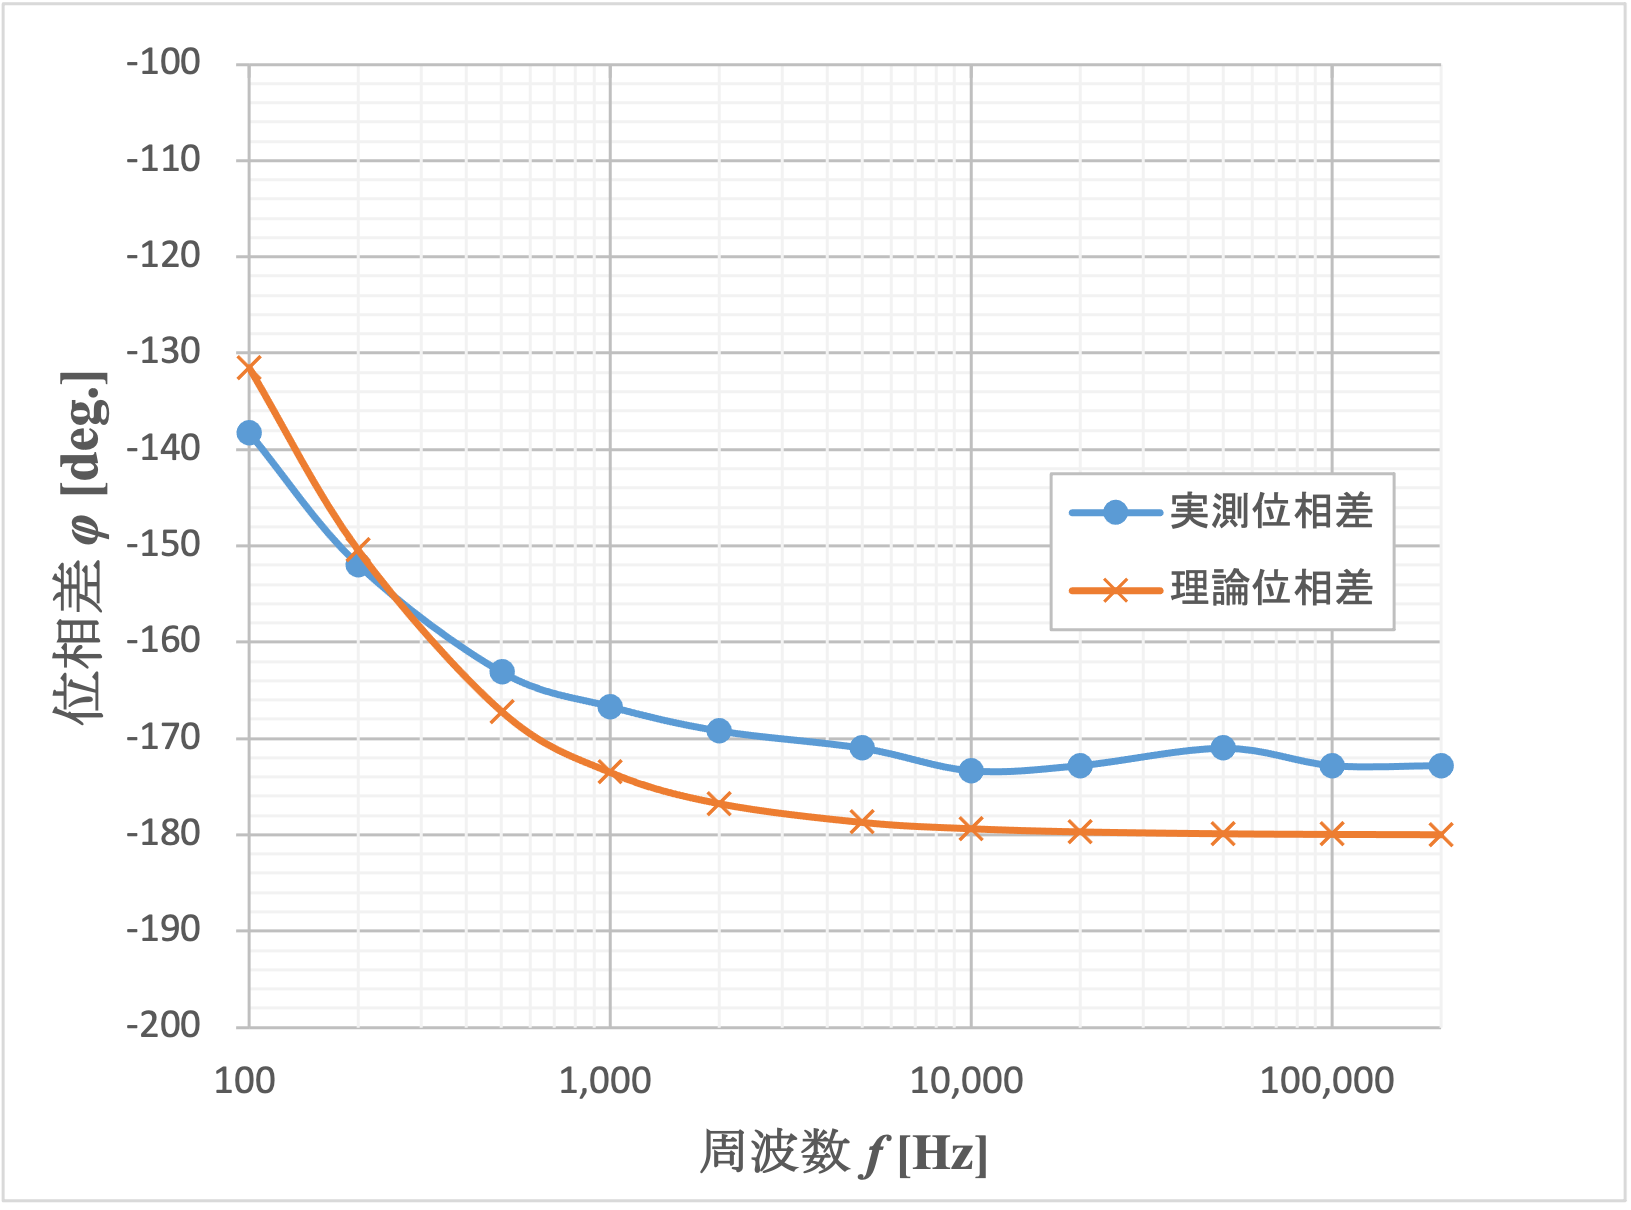
\includegraphics[height=7cm,width=10cm]{syuhasu.png}
  \caption{理論位相差と実測位相差のグラフ}
\end{center}
\end{figure}
\section{考察}
\subsection{(1) $I_C$ - $V_{CE}$ 特性結果において主なパラメータとその影響についての確認できたことを説明する}
$V_{CE}$を4Vに固定したときの測定結果図 4を見る.$I_B$の値は$V_BE$を0~0.55Vに変化させたとき,$I_B$はほとんど変化せず,0mAである.0.55Vを過ぎたあたりから$I_B$が上昇し始める.よって閾値が0.55Vあたりであると考えられる.
次に$V_{CE}$が4Vのときの$I_C$ - $I_B$特性である図 5を確認する.$I_C$ - $I_B$は比例することがわかる.
よって$I_B$が変化すると$I_C$にも変化があることがわかる.
次に$I_B$を固定し,$I_C$ - $V_{CE}$特性結果である図 6を確認すると,$I_B$が10µA,20µA,30µAのときもそれぞれある一定の$V_{CE}$の値を超えると2mA,3.5mA,5mAの値でほとんど一定になっている.
よって$I_C$ - $I_B$,$I_C$ - $V_{CE}$,$I_B$ - $V_{BE}$,$V_{CE}$ - $V_{BE}$が連動しており,$I_B$と$V_{BE}$の値が決まれば$I_C$と$V_{CE}$の値も決まることが確認できる.
\subsection{(2) バイアス回路の理論値と実測値を比較しその結果の報告}
設計したバイアス回路の理論値と実測値である表 5をみて理論値と実測値を比較する.V1は電源電圧なので同等になる.V2の値は多少多く,V3の値は多少少なくなっている.これはR1,R2に設定した抵抗がそれぞれ近い値のものをつかったために変化したものであると考えられる.この結果によってそれぞれV2,V3が関連するものの実測値と理論値に誤差が出ている.
\subsection{(4) 実験3の測定結果から増幅度150倍±10\%,増幅周波数1kHz以上となっているかを確認した結果を述べる.}
図 7: 利得の理想値と実測値のグラフを確認すると,グラフの形は似通ったものになっているが全体的に値が低くなっている.増幅度150倍(43.5dB)の±10\%であるかどうか確認すると41dBあたりを推移しているので設計の範囲内であることがわかる.また1kHz以上で利得の上昇が止まっているため増幅周波数1kHz以上となっているのを確認できる.よって仕様通りに実装できたことが確認できる.
増幅度10\%未満だが差がでたのは実験2の誤差からくるものと考えられる.

\section{まとめ}
NPN型のバイポーラトランジスタによるエミッタ接地電流帰還増幅回路を作成し,信号が増幅されるのを確認した.またバイアス回路の設計をし,トランジスタの増幅作用について検証した.

\begin{thebibliography}{9}
  \bibitem{a} 電気通信大学『アナログ回路実験』2023年,p10$\sim$15
\end{thebibliography}
\end{document}
